\documentclass{article}

\usepackage{fancyhdr}
\usepackage{extramarks}
\usepackage{amsmath}
\usepackage{amsthm}
\usepackage{amsfonts}
\usepackage{tikz}
\usepackage[plain]{algorithm}
\usepackage{algpseudocode}
\usepackage{chngcntr}
\usepackage{mathtools}
\usepackage[utf8]{inputenc}
\usepackage[english]{babel}
\usepackage{thmtools}
\usepackage{mathrsfs}
\usepackage{enumitem}

\declaretheoremstyle[headfont=\scshape,postheadspace=\newline]{mystyle}
\declaretheorem[style=mystyle]{theorem}

\usetikzlibrary{automata,positioning}

%
% Basic Document Settings
%

\topmargin=-0.45in
\evensidemargin=0in
\oddsidemargin=0in
\textwidth=6.5in
\textheight=9.0in
\headsep=0.25in

\linespread{1.1}

\pagestyle{fancy}
\lhead{\hmwkAuthorName}
\chead{\hmwkTitle}
\rhead{\firstxmark}
\lfoot{\lastxmark}
\cfoot{\thepage}

\renewcommand\headrulewidth{0.4pt}
\renewcommand\footrulewidth{0.4pt}

\setlength\parindent{0pt}

%\newtheorem{theorem}{Theorem}[section]
\newtheorem{corollary}{Corollary}[theorem]
\newtheorem{lemma}[theorem]{Lemma}
\theoremstyle{definition}
\newtheorem{definition}{Definition}[section]


%
% Create Problem Sections
%

\newcommand{\enterProblemHeader}[1]{
}

\newcommand{\exitProblemHeader}[1]{
    \nobreak\extramarks{#1 (continued)}{#1 continued on next page\ldots}\nobreak{}
    \stepcounter{#1}
    \nobreak\extramarks{#1}{}\nobreak{}
}

\setcounter{secnumdepth}{0}
\newcounter{partCounter}
\newcounter{homeworkProblemCounter}
\setcounter{homeworkProblemCounter}{1}

%
% Homework Problem Environment
%
% This environment takes an optional argument. When given, it will adjust the
% problem counter. This is useful for when the problems given for your
% assignment aren't sequential. See the last 3 problems of this template for an
% example.
%
\newenvironment{homeworkProblem}[1]{
    \section{#1}
    \setcounter{partCounter}{1}
    \setcounter{equation}{0}
    \setcounter{theorem}{0}
}

%
% Homework Details
%   - Title
%   - Due date
%   - Class
%   - Section/Time
%   - Instructor
%   - Author
%

\newcommand{\hmwkTitle}{MATH 2A: Differential Equations}
\newcommand{\hmwkDueDate}{}
\newcommand{\hmwkClass}{Discrete Mathematics}
\newcommand{\hmwkClassTime}{}
\newcommand{\hmwkClassInstructor}{}
\newcommand{\hmwkAuthorName}{\textbf{Edwin Njinimbam}}

%
% Title Page
%

\title{
    \vspace{2in}
    \textmd{\textbf{\hmwkClass\ \hmwkTitle}}\\
    \vspace{0.1in}\large{\textit{\hmwkClassInstructor\ \hmwkClassTime}}
    \vspace{3in}
}

\author{\hmwkAuthorName}
\date{}

\renewcommand{\part}[1]{\textbf{\large Part \Alph{partCounter}}\stepcounter{partCounter}\\}

%
% Various Helper Commands
%

% Useful for algorithms
\newcommand{\alg}[1]{\textsc{\bfseries \footnotesize #1}}

% For derivatives
\newcommand{\deriv}[2]{\frac{\mathrm{d}{#1}}{\mathrm{d}{#2}}}
\newcommand{\derivs}[2]{\frac{\mathrm{d}^2 {#1}}{\mathrm{d}{#2}^2}}

% For partial derivatives
\newcommand{\pderiv}[2]{\frac{\partial #1}{\partial #2}}
\newcommand{\pderivs}[2]{\frac{\partial^2 #1}{\partial #2^2}}

% Integral dx
\newcommand{\dx}{\mathrm{d}x}

% Alias for the Solution section header
\newcommand{\solution}{\textbf{\large Solution}}

% Probability commands: Expectation, Variance, Covariance, Bias
\newcommand{\E}{\mathrm{E}}
\newcommand{\Var}{\mathrm{Var}}
\newcommand{\Cov}{\mathrm{Cov}}
\newcommand{\Bias}{\mathrm{Bias}}

\newcommand{\ls} {\(\mathcal{LS}(A,\textbf{0})\)}
\newcommand{\nullspace}[1]{\mathcal{N}(#1)}
\newcommand{\p} {$\boxed{1}$~}
\newcommand*\Domain[1]{\in\mathbb{C}^{#1}}
\newcommand{\iu}{{i\mkern1mu}}

\counterwithin*{equation}{section}
\counterwithin*{equation}{subsection}

\newcommand{\matxx}[2] {
\begin{bmatrix}
  #1 \\
  #2 \\
\end{bmatrix}
}

\newcommand{\matxxx}[3] {
\begin{bmatrix}
  #1 \\
  #2 \\
  #3 \\
\end{bmatrix}
}

\newcommand{\matxxxx}[4] {
\begin{bmatrix}
  #1 \\
  #2 \\
  #3 \\
  #4 \\
\end{bmatrix}
}
\newcommand{\matxxxxx}[5] {
\begin{bmatrix}
  #1 \\
  #2 \\
  #3 \\
  #4 \\
  #5 \\
\end{bmatrix}
}

\newcommand{\matxxxxxx}[6] {
\begin{bmatrix}
  #1 \\
  #2 \\
  #3 \\
  #4 \\
  #5 \\
  #6 \\
\end{bmatrix}
}

\newcommand{\arrow}[1] {\xrightarrow[]{\text{#1}}}

\newcommand{\specialcell}[2][c]{%
  \begin{tabular}[#1]{@{}c@{}}#2\end{tabular}}

\newenvironment{solutionToProblem} {

  \bigskip

  \textbf{Solution}
}

\begin{document}

\pagebreak

\begin{homeworkProblem}{Chapter 1 B: Picard's Method}
  \begin{enumerate}[label=(\alph*)]
  \item  Use Picard's method with \(\psi_{0}(x) = 1\) to obtain the next four
    successive approximations of the solution to
    \[y^{\prime}(x) = y(x), \hspace{0.5cm} y(0) = 1\]
    Show that these approximations are just the partial sums of the Maclaurin
    series for the actual solution \(e^x\).

    \begin{solutionToProblem}
      Given that
      \begin{equation}
        y^{\prime}(x) = y(x), \hspace{0.5cm} y(0) = 1
      \end{equation}

      Also given that
      \begin{equation}
        f(x,y) = y(x)
      \end{equation}
      According to picards theorem, we have
      \begin{equation}
        \begin{split}
          \phi_{n+1}(x) & = y_0 + \int^{x}_{x_{0}}{f(t, \phi_{0}(t))}dt \\
          & = 1 + \int^{x}_{0}{1}dt \\
          & = 1 + x
        \end{split}
      \end{equation}

      \begin{equation}
        \begin{split}
          \phi_{2}(x) & = y_0 + \int^{x}_{0}f(t, \phi_1(t))dt \\
          & = 1 + \int^{x}_{0} f(t, \left( 1+t \right))dt \\
          & = 1 + x + \frac{x^2}{2}
        \end{split}
      \end{equation}

      \begin{equation}
        \begin{split}
          \phi_{3}(x) & = y_0 + \int^{x}_{0}f(t, \phi_2(t))dt \\
          & = 1 + \int^{x}_{0} f \left(t, \left( 1+t + \frac{t^2}{2} \right) \right)dt \\
          & = 1 + x + \frac{x^2}{2} + \frac{x^3}{6}
        \end{split}
      \end{equation}

      \begin{equation}
        \begin{split}
          \phi_{4}(x) & = y_0 + \int^{x}_{0}f(t, \phi_3(t))dt \\
          & = 1 + \int^{x}_{0}f \left( t, \left( 1 + t + \frac{t^2}{2} \right) \right)dt \\
          & = 1 + x + \frac{x^2}{2} + \frac{x^3}{6} + \frac{x^4}{24}
        \end{split}
      \end{equation}

      By observing the pattern as \(n\) goes, it is enough to say that
      \[
        \phi_{n}(x) = 1 + x + x^2 + \frac{x^2}{2} + \frac{x^3}{6} + \dots + \frac{x^n}{n!}
      \]

      This is the partial sum of the Maclaurian series of \(e^x\).
    \end{solutionToProblem}

  \item Use Picard's method with \(\psi+{0}(x) = 0\) to obtain the next
    three successive approximations of the solution to the nonlinear problem
    \[
      y^{\prime}(x) = 3x - \left[ y(x)^2 \right], \hspace{0.5cm} y(0) = 0
    \]
    Graph these approximations for \(0 \leq x \leq 1\).

    \begin{solutionToProblem}
      \setcounter{equation}{0}
      \begin{equation}
        \begin{split}
          y(x_1) & = y(x_0) + \int^{x}_{x_0}{f(x,y)dx} \\
          & = f(x,y) = 2x - y^2 \\
          y(0) & = 0
        \end{split}
      \end{equation}
      We assume that \(x_0 = 0, x_1 = 0.25\) then
      \begin{equation}
        \begin{split}
          \phi_1(x) & = y(0) + \int^{x}_{0}{\phi_0(x)dx} = 0 + \int^{x}_{0}{2x - 0}dx = x^2 \\
          \phi_2(x) & = y(0) + \int^{x}_{0}{\phi_1(x)dx} = 0 + \int^{x}_{0}{(2x - x^2)dx} = x^2 - =frac{x^3}{3} \\
          \phi_3(x) & = y(0) + \int^{x}_{0}{\phi_2(x)dx} = 0 + \int^{x}_{0}{(2x - x^2 + \frac{x^3}{3})dx} = x^2 - =frac{x^3}{3} + \frac{x^4}{12} \\
          \phi_4(x) & = y(0) + \int^{x}_{0}{\phi_3(x)dx} = 0 + \int^{x}_{0}{(2x - x^2 + \frac{x^3}{3} - \frac{x^4}{12})dx} = x^2 - =frac{x^3}{3} + \frac{x^4}{12} - \frac{x^5}{60} \\
        \end{split}
      \end{equation}
      If \(x = 0.25, \phi_1(x) = 0.0625, \phi_2(x) = 0.05729, \phi_3(x) =
      0.05761, \phi_4(x) = 0.0576009\).
      Thus, the better approximationn at \(x = 0.25\) is \(0.0576\).

      If \(x = 0.5, \phi_1(x) = 0.25, \phi_2(x) = 0.2083, \phi_3(x) =
      0.203125, \phi_4(x) = 0.21302\).

      If \(x = 0.75, \phi_1(x) = 0.5625, \phi_2(x) = 0.421875, \phi_3(x) =
      0.44824, \phi_4(x) = 0.605419\).

      \begin{center}
        \begin{figure}[h!]
          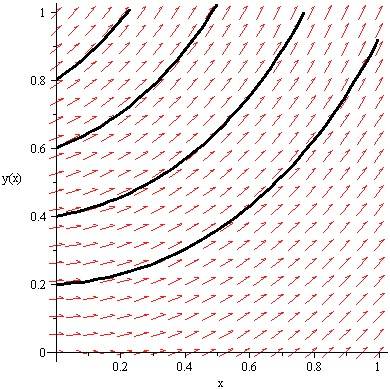
\includegraphics[width=7cm]{chap1b.jpg}
          \caption{}
          \label{fig:chap1b}
        \end{figure}
      \end{center}
    \end{solutionToProblem}

  \item In Problem 29 in Exercises 1.2, we showed that the initial value
    problem
    \[y^{\prime}(x) = 3\left[ y(x)\right]^{2/3}, y(2) = 0\]
    does not have a unique solution. Show that Picard's method beginning
    with \(\psi_{0}(x) = 0\) converges to the solution \(y(x) = 0\),
    whereas Picard's method beginning with \(\psi_{0}(x) = x - 2\)
    converges to the second solution \(y(x) = (x - 2)^{3}\).

    \begin{solutionToProblem}
      \setcounter{equation}{0}
      The given IVP can be written as
      \begin{equation}
        y^{\prime}(t) = f(x, y(x)) \mbox{ where } f(x,y(x)) = 3(y(x))^{2/3}
      \end{equation}

      The first iteration is given by

      \begin{equation}
        \begin{split}
          y_1(x) & = y(2) + \int^{x}_{2} f(u, y(2))du \\
          & = 0 + \int^{t}_{2} f(u, 0)du \\
          & = 0 + \int^{x}_{0} 0du = 0
        \end{split}
      \end{equation}
      If we repeat the procedure, then we get
      \begin{equation}
        y_2(x) = 0
      \end{equation}

      Thus, we get the trivial solution \(y(x) = 0\) for the IVP.

      \bigskip

      Suppose that
      \begin{equation}
        \phi_0(x) = x - 2
      \end{equation}

      Then the first iteration is given by
      \begin{equation}
        \begin{split}
          \phi_1(x) & = \phi_0(x) + \int^{x}_{2} f\left( u, \phi_0(x) \right)du \\
          & = x - 2 + \int^{x}_{2}f(u, x-2)du \\
          & = x - 2 + \int^{x}_{2}{3(x - 2)^{2/3}du} = x - 2 3 \frac{(x-2)^{5/3}}{5/3} \Bigm|_2^x \\
          & = x - 2 + \frac{9}{5}(x-2)^{5/3} = (x-2)\left( 1 + \frac{9}{5}(x-2)^{2/3} \right)
        \end{split}
      \end{equation}

      The second iteration is given by
      \begin{equation}
        \begin{split}
          \phi_2(x) & = \phi_0(x) + \int^{x}_{2}{\left( fu, \phi_1(x) \right)du} \\
          & = x - 2 + \int^{x}_{2}f\left( u, x-2 \right)du \\
          & = x - 2 + \int^{x}_{2}{x - 2 + \frac{9}{5}(x-2)^{5/3}du} = x - 2 + \left( \frac{(x-2)^2}{2} + \frac{9}{5}\frac{(x-2)^{8/3}}{8/3} \Bigm|^{x}_{2} \right) \\
          & = x - 2 =\frac{(x-2)^{2}}{2} + \frac{27}{40}(x-2)^{8/3}
        \end{split}
      \end{equation}
    \end{solutionToProblem}
  \end{enumerate}
\end{homeworkProblem}

\pagebreak

\begin{homeworkProblem}{The Phase Line}
  \begin{enumerate}[label=(\alph*)]
  \item The slopes in the direction field are all identical along horizontal
    lines.

    \begin{solutionToProblem}
    \end{solutionToProblem}
    
  \item New solutions can be generated from old ones by time shifting [i.e.,
    replacing \(y(t)\) with \(y(t-t_0)\).]

    \begin{solutionToProblem}
    \end{solutionToProblem}
        
  \item Sketch the phase line for \(y^{\prime} = (y - 1)(y - 2)(y - 3)\) and
    state the nature of its equilibria.

    \begin{solutionToProblem}
    \end{solutionToProblem}
    
  \item Use the phase line for \(y^{\prime} = -(y - 1)^{5/3}(y - 2)^2(y -
    3)\) to predict the asymtotic behavior as \(t \rightarrow \infty\) of the
    solution satisfying \(y(0) = 2.1\).
    \begin{solutionToProblem}
    \end{solutionToProblem}
    
  \item Sketch the phase line for \(y^{\prime} = y{\sin{y}}\) and state the
    nature of its equilibria.
    \begin{solutionToProblem}
    \end{solutionToProblem}
    
  \item Sketch the phase lines for \(y^{\prime} = y \sin{y} + 0.1\) and
    \(y^{\prime} = y\sin{y} - 0.1\). Discuss the effect of the small
    perturbation \(\pm 0.1\) on the equilibria.
    \begin{solutionToProblem}
    \end{solutionToProblem}
  \end{enumerate}
\end{homeworkProblem}
\end{document}
